\documentclass{beamer}

\usetheme{Boadilla}
% \usecolortheme{beaver} % --- We are replacing this with our own theme below ---

\usepackage{amsmath}
\usepackage{amssymb}
\usepackage{graphicx}
\usepackage{physics}
\usepackage{mathtools}
\usepackage{siunitx}
\usepackage{tikz}
\usetikzlibrary{positioning, shapes.geometric, arrows.meta}
\usepackage{booktabs}
\usepackage{lmodern}
\usepackage{setspace}
\onehalfspacing
\usepackage[bottom]{footmisc}

% --- CUSTOM COLOR THEME SETUP ---

% 1. Define your new colors using Hex codes
\definecolor{ULBBlue}{HTML}{0D47A1}
\definecolor{ULBTeal}{HTML}{4DB6AC}
\definecolor{VUBOrange}{HTML}{E87722}
\definecolor{AlertColor}{HTML}{D32F2F}
\definecolor{LightGray}{HTML}{F5F5F5}


% 2. Apply these colors to Beamer's elements
\setbeamercolor{palette primary}{bg=ULBBlue, fg=white}
\setbeamercolor{palette secondary}{bg=VUBOrange, fg=white}
\setbeamercolor{palette tertiary}{bg=ULBBlue, fg=white}
\setbeamercolor{palette quaternary}{bg=VUBOrange, fg=white}

\setbeamercolor{structure}{fg=ULBBlue} % This is a key color for many elements
\setbeamercolor{titlelike}{bg=ULBBlue, fg=white}
\setbeamercolor{frametitle}{bg=ULBBlue, fg=white}
\setbeamercolor{title}{use=structure,fg=white,bg=structure.fg}

\setbeamercolor{normal text}{fg=black, bg=white}
\setbeamercolor{block title}{use=structure,fg=white,bg=structure.fg}
\setbeamercolor{block body}{bg=LightGray}
\setbeamercolor{alerted text}{fg=AlertColor}

% --- END OF CUSTOM COLOR THEME ---

% --- Command to automatically create a title slide for each section ---
\AtBeginSection[]{
	\begin{frame}
		\vfill
		\centering
		\begin{beamercolorbox}[sep=8pt,center,shadow=true,rounded=true]{title}
			\usebeamerfont{title}\insertsectionhead\par%
		\end{beamercolorbox}
		\vfill
	\end{frame}
}
% --- END of command ---


\title[Over-the-Ground Model \& Impulse Response]{Question 2: Over-the-Ground Propagation, Path Loss, and Channel Impulse Response}
\subtitle{Demonstration and Application to Half-Wave Dipoles}
\author{Cédric Sipakam}
\institute{ULB | VUB \\
	\vspace{1.5em}
	ELEC-H415: Communication Channels}
\date{2025}


\setbeamertemplate{footline}
{
	\leavevmode%
	\hbox{%
		\begin{beamercolorbox}[wd=.5\paperwidth,ht=2.25ex,dp=1ex,left]{author in head/foot}%
			\hspace*{2ex}\usebeamerfont{title in head/foot}\insertshorttitle%
		\end{beamercolorbox}%
		\begin{beamercolorbox}[wd=.5\paperwidth,ht=2.25ex,dp=1ex,right]{title in head/foot}%
			\usebeamerfont{page number in head/foot}\insertframenumber{} / \inserttotalframenumber\hspace*{2ex}%
		\end{beamercolorbox}%
	}%
	\vskip0pt%
}



\begin{document}
	\begin{frame}
		\begin{figure}
			\centering
			
\includegraphics[width=0.7\linewidth]{pictures/logos}
		\end{figure}
		\titlepage
	\end{frame}
	
	\begin{frame}{Outline}
		\tableofcontents
	\end{frame}
	
	\section{The Over-the-Ground Propagation Model}
	
	\begin{frame}{Motivation: Beyond Free Space}
		\begin{itemize}
			\item The Friis formula describes propagation in free space, but most terrestrial communications involve reflections, particularly from the ground.
			\item The \textbf{over-the-ground model}, also known as the two-ray model, is a fundamental physical model that accounts for the interference between the direct (LOS) path and the ground-reflected path.
		\end{itemize}
	\end{frame}
	
	\begin{frame}{Motivation: Beyond Free Space}
		\begin{figure}
			\centering
			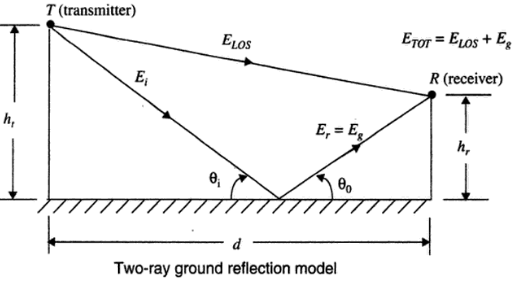
\includegraphics[width=0.7\linewidth]{"pictures/two-ray-geometry.png"}
			\caption{Geometry of the two-ray (over-the-ground) propagation model.}
		\end{figure}
	\end{frame}
	
	\begin{frame}{Model Setup and Assumptions}
		\begin{itemize}
			\item We consider two propagation paths:
			\begin{itemize}
				\item A direct Line-of-Sight (LOS) path of length $d_1$.
				\item A single ground-reflected path of length $d_2$.
			\end{itemize}
			\item \textbf{Assumptions}:
			\begin{itemize}
				\item The antennas (TX and RX) are vertically polarized (z-directed) and omnidirectional in the horizontal (xy) plane.
				\item The ground is modeled as a smooth, planar surface with a relative permittivity $\epsilon_r$.
				\item We use ray-tracing and geometrical optics to determine the paths.
			\end{itemize}
		\end{itemize}
	\end{frame}
	
	\begin{frame}{Formulating the Received Power}
		\begin{itemize}
			\item The total received electric field $\underline{\vec{E}}_{tot}$ is the coherent sum of the fields from the two paths:
			\[ \underline{\vec{E}}_{tot} = \underline{\vec{E}}_{1} + \underline{\vec{E}}_{2} \]
			\item The LOS field $\underline{\vec{E}}_{1}$ and the reflected field $\underline{\vec{E}}_{2}$ are given by:
			\[ \underline{\vec{E}}_{1} = E_0 \frac{e^{-j\beta d_1}}{d_1} \vec{1}_z \quad , \quad \underline{\vec{E}}_{2} = \Gamma_{\perp}(\theta_i) E_0 \frac{e^{-j\beta d_2}}{d_2} \vec{1}_z \]
			where $\Gamma_{\perp}(\theta_i)$ is the reflection coefficient for perpendicular (vertical) polarization.
		\end{itemize}
	\end{frame}
	
	\begin{frame}{Formulating the Received Power}
		\begin{block}{Reflection Coefficient}
			The coefficient depends on the angle of incidence $\theta_i$ and the ground's permittivity $\epsilon_r$:
			\[ \Gamma_{\perp}(\theta_i) = \frac{\cos\theta_i - \sqrt{\epsilon_r - \sin^2\theta_i}}{\cos\theta_i + \sqrt{\epsilon_r - \sin^2\theta_i}} \]
		\end{block}
	\end{frame}
	
	\begin{frame}{Deriving Total Received Power}
		\begin{itemize}
			\item The open-circuit voltage $V_{oc}$ at the receiver is the sum of contributions from both paths:
			\[ \underline{V}_{oc} \propto h_{e\perp}^{TX} h_{e\perp}^{RX} \left( \frac{e^{-j\beta d_1}}{d_1} + \Gamma_{\perp} \frac{e^{-j\beta d_2}}{d_2} \right) \]
			
		\end{itemize}
		
	\end{frame}
	
	\begin{frame}{Deriving Total Received Power}
		\begin{itemize}
			
			\item Using the relationship between received power, voltage, and antenna parameters, we can write the total received power $P_{RX}$ as:
			\[ P_{RX} = P_{TX} G_{TX} G_{RX} \left( \frac{\lambda}{4\pi} \right)^2 \left| \frac{e^{-j\beta d_1}}{d_1} + \Gamma_{\perp} \frac{e^{-j\beta d_2}}{d_2} \right|^2 \]
		\end{itemize}
		\begin{alertblock}{Result}
			This relation is the complete two-ray model. It captures the constructive and destructive interference between the two paths, leading to oscillations in received power as a function of distance.
		\end{alertblock}
	\end{frame}
	
	\section{Large Distance Approximation \& Path Loss}
	
	\begin{frame}{Simplifying for Large Distances}
		\begin{itemize}
			\item In many macro-cell scenarios, the horizontal distance $d$ is much larger than the antenna heights ($d \gg h_{TX}, h_{RX}$).
			\item This allows for several simplifications:
			\begin{itemize}
				\item \textbf{Grazing Incidence}: The reflection angle $\theta_i \to \pi/2$, which makes the reflection coefficient $\Gamma_{\perp} \approx -1$.
				\item \textbf{Amplitudes}: For the amplitude terms, the path lengths are nearly equal: $d_1 \approx d_2 \approx d$.
				\item \textbf{Phases}: For the phase terms, the small difference between $d_1$ and $d_2$ is critical and must be retained.
			\end{itemize}
		\end{itemize}
	\end{frame}
	
	\begin{frame}{Derivation of the $d^{-4}$ Law}
		\begin{itemize}
			\item Applying the approximations $\Gamma_{\perp} \approx -1$ and $d_1 \approx d_2 \approx d$ to the amplitude part of the $P_{RX}$ relation gives:
			\[ P_{RX} \approx P_{TX} G_{TX} G_{RX} \left( \frac{\lambda}{4\pi d} \right)^2 \left| e^{-j\beta d_1} - e^{-j\beta d_2} \right|^2 \]
			\item The magnitude term can be rewritten using Euler's relation:
			\[ |e^{-j\beta d_1} - e^{-j\beta d_2}|^2 = |e^{-j\beta (d_1+d_2)/2}(e^{j\beta (d_2-d_1)/2} - e^{-j\beta (d_2-d_1)/2})|^2 \]
			\[ = |2j \sin\left(\frac{\beta(d_2-d_1)}{2}\right)|^2 = 4\sin^2\left(\frac{\beta(d_2-d_1)}{2}\right) \]
			
		\end{itemize}
	\end{frame}
	
	\begin{frame}{Derivation of the $d^{-4}$ Law}
		\begin{itemize}
			\item This yields:
			\[ P_{RX} \approx P_{TX} G_{TX} G_{RX} \left( \frac{\lambda}{4\pi d} \right)^2 \cdot 4\sin^2\left(\frac{\beta(d_2-d_1)}{2}\right) \]
			
			\item The path length difference $\Delta d = d_2 - d_1$ can be approximated using Taylor expansion:
			\[ d_1 = \sqrt{d^2 + (h_{TX}-h_{RX})^2} \approx d \left(1 + \frac{(h_{TX}-h_{RX})^2}{2d^2}\right) \]
			\[ d_2 = \sqrt{d^2 + (h_{TX}+h_{RX})^2} \approx d \left(1 + \frac{(h_{TX}+h_{RX})^2}{2d^2}\right) \]
			
		\end{itemize}
	\end{frame}
	
	\begin{frame}{Derivation of the $d^{-4}$ Law}
		\[ \implies \Delta d = d_2 - d_1 \approx \frac{2 h_{TX} h_{RX}}{d} \]
		\begin{itemize}
			
			\item Since $\Delta d$ is small, we use the small-angle approximation $\sin(x) \approx x$:
			\[ \sin^2\left(\frac{\beta(d_2-d_1)}{2}\right) \approx \left(\frac{\beta \Delta d}{2}\right)^2 = \left(\frac{2\pi}{\lambda} \frac{h_{TX}h_{RX}}{d}\right)^2 \]
			\item Substituting this back into the $P_{RX}$ expression gives the result:
			\[ P_{RX}(d) \approx P_{TX} G_{TX} G_{RX} \frac{h_{TX}^2 h_{RX}^2}{d^4} \]
		\end{itemize}
	\end{frame}
	
	\begin{frame}{The Canonical Path Loss Model}
		\begin{itemize}
			\item The large distance approximation shows that $P_{RX} \propto d^{-4}$.
			\item This fits the general \textbf{canonical path loss model}:
			\[ \ll P_{RX}(d)\gg[\text{dBm}] = \ll P_{RX}(d_{0})\gg[\text{dBm}] - 10n \log_{10}\left(\frac{d}{d_0}\right) \]
			\item For the over-the-ground model at large distances, the \textbf{path loss exponent} is $n=4$.
		\end{itemize}
	\end{frame}
	
	\begin{frame}{The Canonical Path Loss Model}
		\begin{figure}
			\centering
			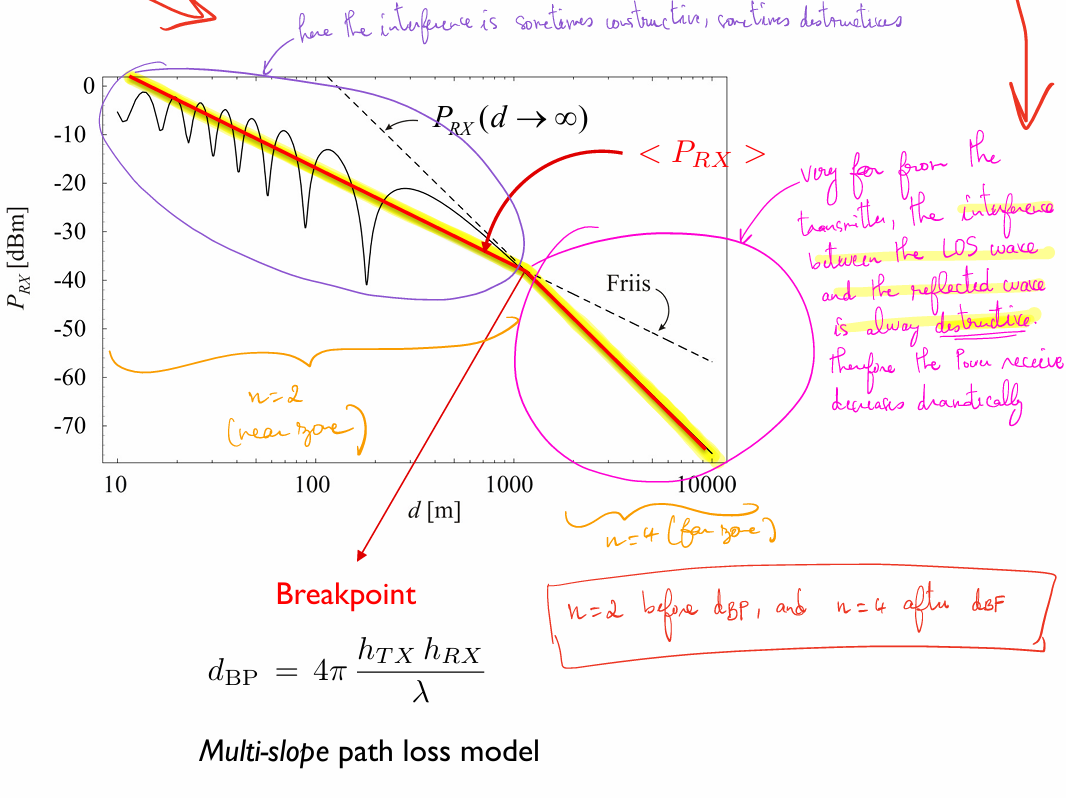
\includegraphics[width=0.65\linewidth]{"pictures/pathloss-plot.png"}
			\caption{Received power vs. distance, showing the Friis model ($n=2$), the full two-ray model, and the large distance approximation ($n=4$).}
		\end{figure}
/	\end{frame}
	
	\section{Impulse Response for Dipole Antennas}
	
	\begin{frame}{Physical Impulse Response}
		\begin{itemize}
			\item The physical channel is described by its time-varying impulse response, $h(\tau, t)$. For a static scenario, it is $h(\tau)$.
			\item It is a sum of delayed Dirac delta functions, each representing a multipath component (MPC):
			\[ h(\tau) = \sum_{n=1}^{N} \alpha_n \delta(\tau - \tau_n) \]
			\item For the over-the-ground model, we have $N=2$ MPCs.
			\item The complex amplitude $\alpha_n = a_n e^{j\phi_n}e^{-j2\pi f_c \tau_n}$ represents the gain and phase shift of each path at the carrier frequency $f_c$.
		\end{itemize}
	\end{frame}
	
	\begin{frame}{Wideband Impulse Response}
		\begin{itemize}
			\item A wideband system has enough time resolution to distinguish the two paths.
			\item The impulse response consists of two distinct Dirac deltas:
			\[ h_{WB}(\tau) = \alpha_1 \delta(\tau - \tau_1) + \alpha_2 \delta(\tau - \tau_2) \]
			
		\end{itemize}
	\end{frame}
	
	\begin{frame}{Wideband Impulse Response}
		\begin{itemize}
			\item The parameters are:
			\begin{itemize}
				\item \textbf{Delays}: $\tau_1 = d_1/c$ and $\tau_2 = d_2/c$.
				\item \textbf{Amplitudes}: The $\alpha_n$ terms are derived from the terms in the received voltage expression. Let $K$ be a constant representing transmit power and antenna properties. Then:
				\[ \alpha_1 = K \frac{e^{-j2\pi f_c \tau_1}}{d_1} \]
				\[ \alpha_2 = K \cdot \Gamma_{\perp}(\theta_i) \frac{e^{-j2\pi f_c \tau_2}}{d_2} \]
				where $\Gamma_{\perp}$ is the reflection coefficient for z-directed (vertical) dipoles.
			\end{itemize}
		\end{itemize}
	\end{frame}
	
	
	\begin{frame}{Narrowband Impulse Response}
		\begin{itemize}
			\item A system is narrowband if its time resolution $\Delta\tau \approx 1/B$ is much larger than the channel's delay spread $\sigma_\tau = \tau_2 - \tau_1$.
			\item In this case, the receiver cannot distinguish between the LOS and reflected paths.
			\item The two MPCs merge into a single, effective tap at $\tau=0$.
			
		\end{itemize}
	\end{frame}
	
	\begin{frame}{Narrowband Impulse Response}
		\begin{itemize}
			\item The narrowband channel coefficient, $h_{NB}$, is the coherent sum of the complex amplitudes of all MPCs:
			\[ h_{NB} = \sum_{n=1}^{2} \alpha_n = \alpha_1 + \alpha_2 \]
			\[ h_{NB} = K \left( \frac{e^{-j2\pi f_c \tau_1}}{d_1} + \Gamma_{\perp}(\theta_i) \frac{e^{-j2\pi f_c \tau_2}}{d_2} \right) \]
			\item The impulse response is then simply:
			\[ h_{NB}(\tau) = h_{NB} \cdot \delta(\tau) \]
		\end{itemize}
	\end{frame}
	
	\section{Conclusion}
	
	\begin{frame}{Summary}
		\begin{block}{Over-the-Ground Model}
			\begin{itemize}
				\item Provides a more realistic propagation model than free-space by including a ground-reflected path.
				\item Correctly predicts interference phenomena (fading nulls) as a function of distance.
			\end{itemize}
		\end{block}
	\end{frame}
	
	\begin{frame}{Summary}
		\begin{block}{Path Loss}
			\begin{itemize}
				\item At large distances, the two-ray model simplifies to a power decay of $P_{RX} \propto d^{-4}$.
				\item This corresponds to a canonical path loss model with an exponent of $n=4$.
			\end{itemize}
		\end{block}
	\end{frame}
	
	\begin{frame}{Summary}
		\begin{block}{Channel Impulse Response}
			\begin{itemize}
				\item In a wideband view, the channel is represented by two distinct paths with different delays and amplitudes.
				\item In a narrowband view, these paths are unresolvable and combine into a single complex coefficient, leading to flat fading.
			\end{itemize}
		\end{block}
	\end{frame}
	
	\begin{frame}{Conclusion}
		\begin{alertblock}{From Physics to Models}
			The demonstration of the over-the-ground model shows how a simple physical scenario (a direct and a reflected ray) leads to powerful and widely applicable concepts in wireless communications.
			
			It explains the origin of a non-trivial path loss exponent ($n=4$) and provides a clear physical basis for the distinction between wideband (frequency-selective) and narrowband (flat-fading) channel models. Understanding this foundation is crucial for designing and predicting the performance of real-world wireless systems.
		\end{alertblock}
	\end{frame}
	
	\section{Thank You}
	
\end{document}
